\clearpage
\section{候选过滤、加权抽取与收藏冷却}
\label{sec:design-drawing}
相遇抽取分为资格筛选和加权抽样两个阶段。用户的匹配标签提取完成后，系统才开始筛选候选对象。真人候选要排除本人、匹配资料未就绪或关闭纸条接收的账号，以及已经建立会话或任一方向有待回应纸条的对象。虚拟候选排除已屏蔽人物。两类对象分别识别，都要再排除已收藏、还在冷却期或匹配分低于60的对象。

通过筛选后，用匹配分 $w_i=M(a,i)$ 当权重。匹配分越高，抽中概率越大。
\begin{equation}
P(i\mid\text{本次候选池})=\frac{w_i}{\sum_jw_j}.\label{eq:design-draw}
\end{equation}
假设剩下三位候选，分数为60、80、100，抽中概率分别是25\%、$1/3$ 和 $5/12$。卡片颜色显示的是匹配档位。

\begin{figure}[H]
\centering
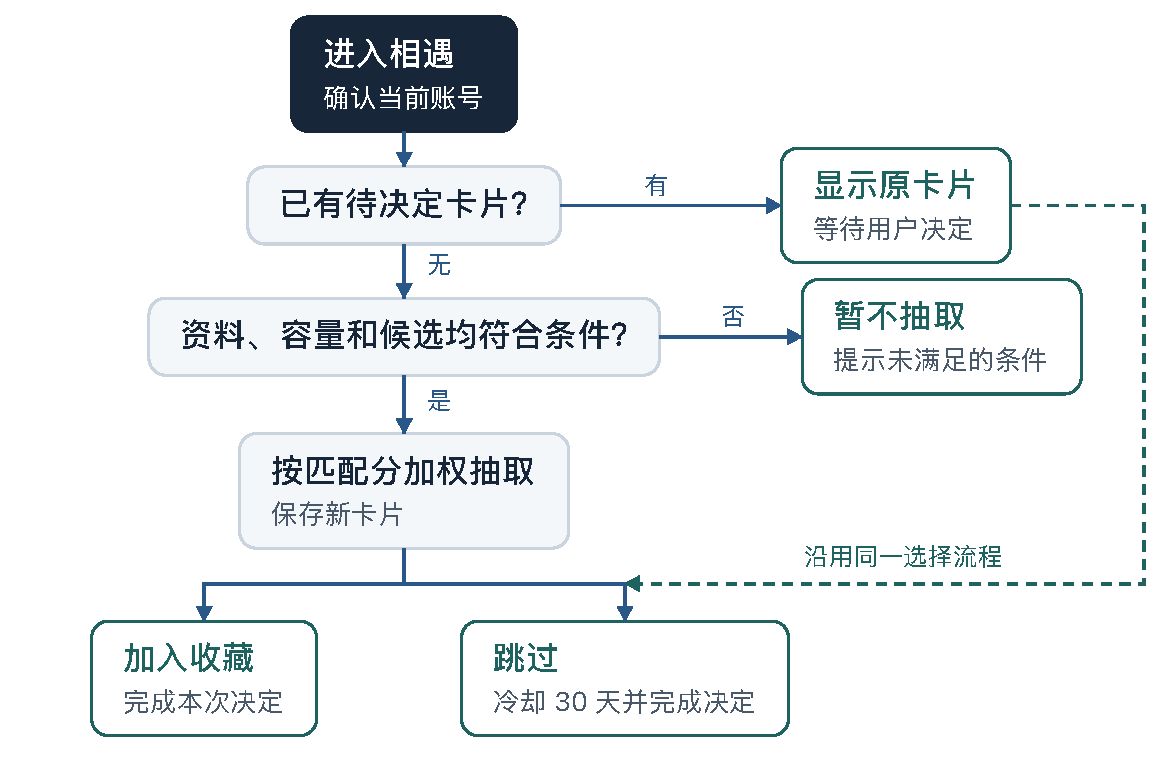
\includegraphics[width=\linewidth]{assets/design/draw-flow.pdf}
\caption{待决定卡片复用与收藏、跳过流程}\label{fig:design-draw-flow}
\end{figure}

当前演示不限制每日抽取次数。系统为每个账号保留至多一张待处理卡片，重复请求返回同一张卡，用户选择收藏或跳过后才允许抽取下一张。最多收藏5位，保存时还要确认真人账号仍可用。资料未就绪、收藏已满或找不到合适候选时，页面会显示具体原因。跳过或移除收藏会让该对象进入30天冷却，已有真人会话和虚拟交流历史仍能打开。

